\documentclass[]{article}
\usepackage{lmodern}
\usepackage{amssymb,amsmath}
\usepackage{ifxetex,ifluatex}
\usepackage{fixltx2e} % provides \textsubscript
\ifnum 0\ifxetex 1\fi\ifluatex 1\fi=0 % if pdftex
  \usepackage[T1]{fontenc}
  \usepackage[utf8]{inputenc}
\else % if luatex or xelatex
  \ifxetex
    \usepackage{mathspec}
  \else
    \usepackage{fontspec}
  \fi
  \defaultfontfeatures{Ligatures=TeX,Scale=MatchLowercase}
\fi
% use upquote if available, for straight quotes in verbatim environments
\IfFileExists{upquote.sty}{\usepackage{upquote}}{}
% use microtype if available
\IfFileExists{microtype.sty}{%
\usepackage{microtype}
\UseMicrotypeSet[protrusion]{basicmath} % disable protrusion for tt fonts
}{}
\usepackage[margin=1in]{geometry}
\usepackage{hyperref}
\hypersetup{unicode=true,
            pdftitle={DDSAnalytics: Case Study 2},
            pdfauthor={David Coppiellie},
            pdfborder={0 0 0},
            breaklinks=true}
\urlstyle{same}  % don't use monospace font for urls
\usepackage{graphicx,grffile}
\makeatletter
\def\maxwidth{\ifdim\Gin@nat@width>\linewidth\linewidth\else\Gin@nat@width\fi}
\def\maxheight{\ifdim\Gin@nat@height>\textheight\textheight\else\Gin@nat@height\fi}
\makeatother
% Scale images if necessary, so that they will not overflow the page
% margins by default, and it is still possible to overwrite the defaults
% using explicit options in \includegraphics[width, height, ...]{}
\setkeys{Gin}{width=\maxwidth,height=\maxheight,keepaspectratio}
\IfFileExists{parskip.sty}{%
\usepackage{parskip}
}{% else
\setlength{\parindent}{0pt}
\setlength{\parskip}{6pt plus 2pt minus 1pt}
}
\setlength{\emergencystretch}{3em}  % prevent overfull lines
\providecommand{\tightlist}{%
  \setlength{\itemsep}{0pt}\setlength{\parskip}{0pt}}
\setcounter{secnumdepth}{0}
% Redefines (sub)paragraphs to behave more like sections
\ifx\paragraph\undefined\else
\let\oldparagraph\paragraph
\renewcommand{\paragraph}[1]{\oldparagraph{#1}\mbox{}}
\fi
\ifx\subparagraph\undefined\else
\let\oldsubparagraph\subparagraph
\renewcommand{\subparagraph}[1]{\oldsubparagraph{#1}\mbox{}}
\fi

%%% Use protect on footnotes to avoid problems with footnotes in titles
\let\rmarkdownfootnote\footnote%
\def\footnote{\protect\rmarkdownfootnote}

%%% Change title format to be more compact
\usepackage{titling}

% Create subtitle command for use in maketitle
\providecommand{\subtitle}[1]{
  \posttitle{
    \begin{center}\large#1\end{center}
    }
}

\setlength{\droptitle}{-2em}

  \title{DDSAnalytics: Case Study 2}
    \pretitle{\vspace{\droptitle}\centering\huge}
  \posttitle{\par}
    \author{David Coppiellie}
    \preauthor{\centering\large\emph}
  \postauthor{\par}
      \predate{\centering\large\emph}
  \postdate{\par}
    \date{12/5/2019}


\begin{document}
\maketitle

\hypertarget{introduction}{%
\subsection{Introduction}\label{introduction}}

\begin{itemize}
\tightlist
\item
  Project 2: DDSAnalytics

  \begin{itemize}
  \tightlist
  \item
    Developed and Presented By: David Coppiellie Goals:
  \item
    Achieve 60\% Sensitivity and 60\% Specificty for Predictive Model on
    Attrittion
  \item
    Develop Logistic Regression Model with RSME \textless{} \$3,000
    Presentation:
    \href{https://www.youtube.com/watch?v=XnEKwkAcfhg\&t=10s}{Project 2}
  \end{itemize}
\end{itemize}

\hypertarget{review-of-tasks}{%
\subsection{Review of Tasks}\label{review-of-tasks}}

\begin{itemize}
\tightlist
\item
  Explore Employee Data Provided by DDSAnalytics
\item
  Analyze Employee Data to Understand ``Attrition''
\item
  Provide a Predictive Model for ``Attrition''
\item
  Provide a Predictive Model for ``MonthlyIncome''
\end{itemize}

\hypertarget{exploration-of-employeee-data}{%
\subsection{Exploration of Employeee
Data}\label{exploration-of-employeee-data}}

\begin{itemize}
\tightlist
\item
  Analyze Data Structure
\item
  Analyze Correlations between Numeric Variables
\item
  Analyze Correlations between Numeric and Categorical Variables
\item
  Analyze Correlations between Categorical variables
\item
  Eliminate Variables that Overfit a Model
\item
  Compare k-NN and NaiveBayes Classifiers on ``Attrition''
\item
  Predict ``MontlyIncome'' with Linear Regression Analysis
\end{itemize}

\hypertarget{data-structure}{%
\subsection{Data Structure}\label{data-structure}}

\begin{verbatim}
## 'data.frame':    870 obs. of  36 variables:
##  $ ID                      : int  1 2 3 4 5 6 7 8 9 10 ...
##  $ Age                     : int  32 40 35 32 24 27 41 37 34 34 ...
##  $ Attrition               : Factor w/ 2 levels "No","Yes": 1 1 1 1 1 1 1 1 1 1 ...
##  $ BusinessTravel          : Factor w/ 3 levels "Non-Travel","Travel_Frequently",..: 3 3 2 3 2 2 3 3 3 2 ...
##  $ DailyRate               : int  117 1308 200 801 567 294 1283 309 1333 653 ...
##  $ Department              : Factor w/ 3 levels "Human Resources",..: 3 2 2 3 2 2 2 3 3 2 ...
##  $ DistanceFromHome        : int  13 14 18 1 2 10 5 10 10 10 ...
##  $ Education               : int  4 3 2 4 1 2 5 4 4 4 ...
##  $ EducationField          : Factor w/ 6 levels "Human Resources",..: 2 4 2 3 6 2 4 2 2 6 ...
##  $ EmployeeCount           : int  1 1 1 1 1 1 1 1 1 1 ...
##  $ EmployeeNumber          : int  859 1128 1412 2016 1646 733 1448 1105 1055 1597 ...
##  $ EnvironmentSatisfaction : int  2 3 3 3 1 4 2 4 3 4 ...
##  $ Gender                  : Factor w/ 2 levels "Female","Male": 2 2 2 1 1 2 2 1 1 2 ...
##  $ HourlyRate              : int  73 44 60 48 32 32 90 88 87 92 ...
##  $ JobInvolvement          : int  3 2 3 3 3 3 4 2 3 2 ...
##  $ JobLevel                : int  2 5 3 3 1 3 1 2 1 2 ...
##  $ JobRole                 : Factor w/ 9 levels "Healthcare Representative",..: 8 6 5 8 7 5 7 8 9 1 ...
##  $ JobSatisfaction         : int  4 3 4 4 4 1 3 4 3 3 ...
##  $ MaritalStatus           : Factor w/ 3 levels "Divorced","Married",..: 1 3 3 2 3 1 2 1 2 2 ...
##  $ MonthlyIncome           : int  4403 19626 9362 10422 3760 8793 2127 6694 2220 5063 ...
##  $ MonthlyRate             : int  9250 17544 19944 24032 17218 4809 5561 24223 18410 15332 ...
##  $ NumCompaniesWorked      : int  2 1 2 1 1 1 2 2 1 1 ...
##  $ Over18                  : Factor w/ 1 level "Y": 1 1 1 1 1 1 1 1 1 1 ...
##  $ OverTime                : Factor w/ 2 levels "No","Yes": 1 1 1 1 2 1 2 2 2 1 ...
##  $ PercentSalaryHike       : int  11 14 11 19 13 21 12 14 19 14 ...
##  $ PerformanceRating       : int  3 3 3 3 3 4 3 3 3 3 ...
##  $ RelationshipSatisfaction: int  3 1 3 3 3 3 1 3 4 2 ...
##  $ StandardHours           : int  80 80 80 80 80 80 80 80 80 80 ...
##  $ StockOptionLevel        : int  1 0 0 2 0 2 0 3 1 1 ...
##  $ TotalWorkingYears       : int  8 21 10 14 6 9 7 8 1 8 ...
##  $ TrainingTimesLastYear   : int  3 2 2 3 2 4 5 5 2 3 ...
##  $ WorkLifeBalance         : int  2 4 3 3 3 2 2 3 3 2 ...
##  $ YearsAtCompany          : int  5 20 2 14 6 9 4 1 1 8 ...
##  $ YearsInCurrentRole      : int  2 7 2 10 3 7 2 0 1 2 ...
##  $ YearsSinceLastPromotion : int  0 4 2 5 1 1 0 0 0 7 ...
##  $ YearsWithCurrManager    : int  3 9 2 7 3 7 3 0 0 7 ...
\end{verbatim}

\hypertarget{numeric-variable-analysis}{%
\subsection{Numeric Variable Analysis}\label{numeric-variable-analysis}}

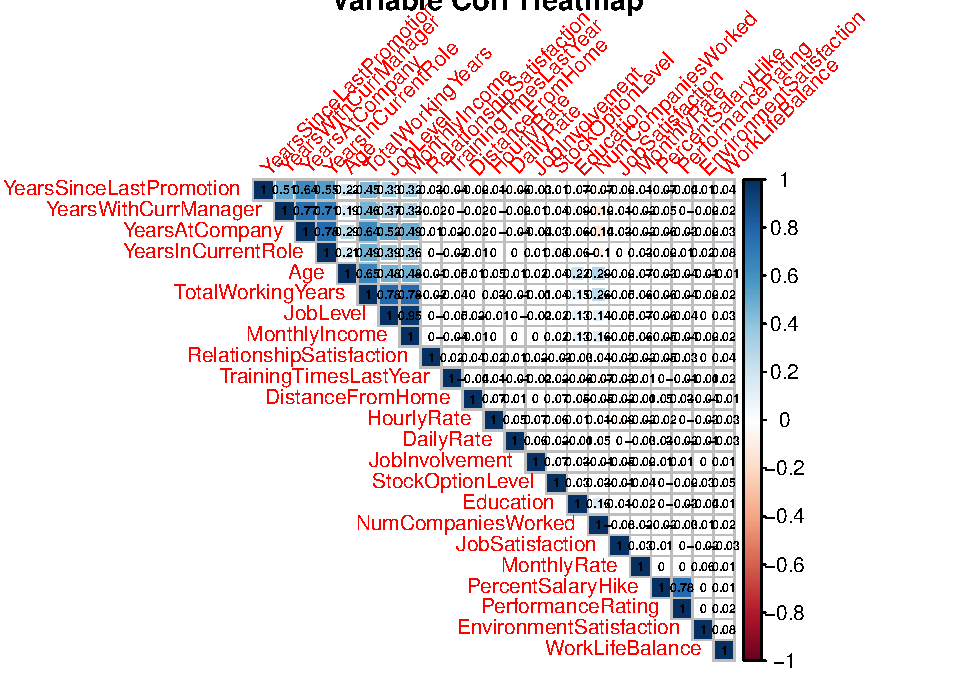
\includegraphics{PresentationPDF_files/figure-latex/unnamed-chunk-2-1.pdf}

\hypertarget{numeric-and-categorical-variable-analysis}{%
\subsection{Numeric and Categorical Variable
Analysis}\label{numeric-and-categorical-variable-analysis}}

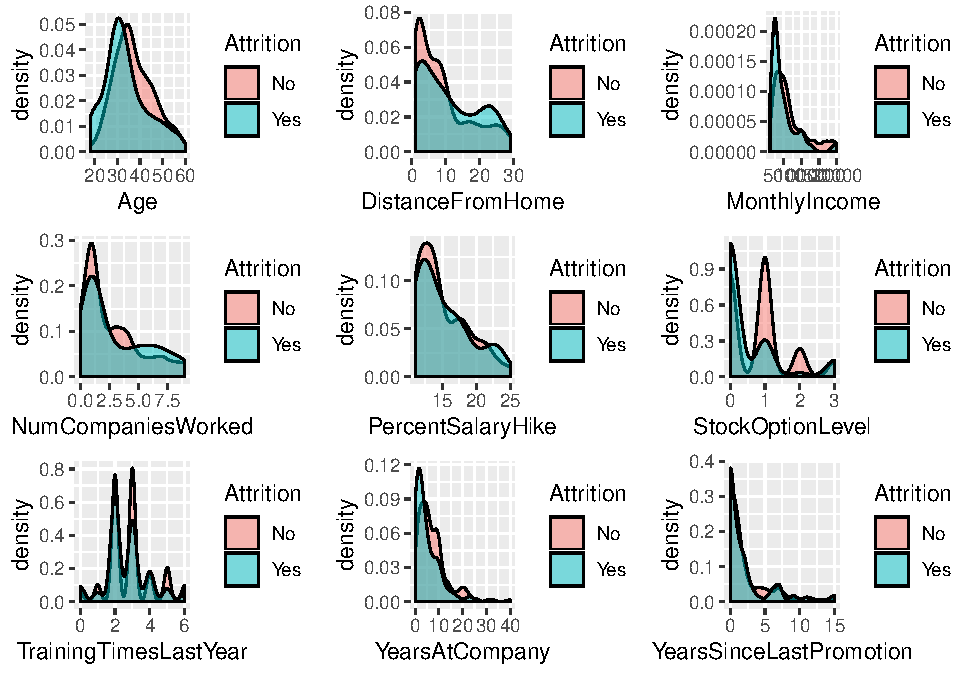
\includegraphics{PresentationPDF_files/figure-latex/unnamed-chunk-3-1.pdf}

\hypertarget{categorical-variable-analysis}{%
\subsection{Categorical Variable
Analysis}\label{categorical-variable-analysis}}

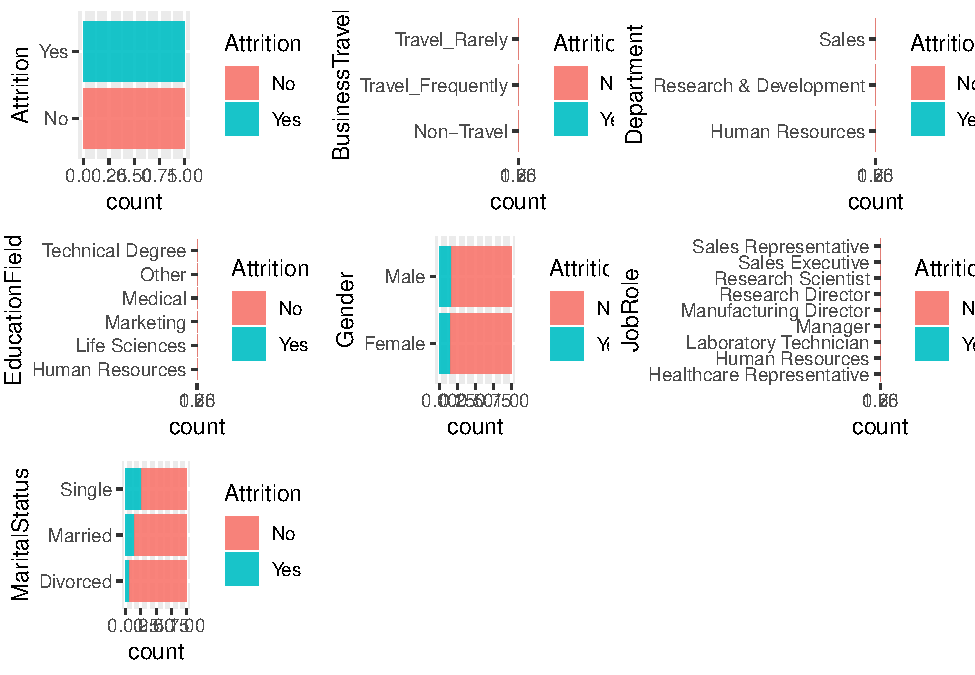
\includegraphics{PresentationPDF_files/figure-latex/unnamed-chunk-4-1.pdf}

\hypertarget{check-for-overfit-variables}{%
\subsection{Check for Overfit
Variables}\label{check-for-overfit-variables}}

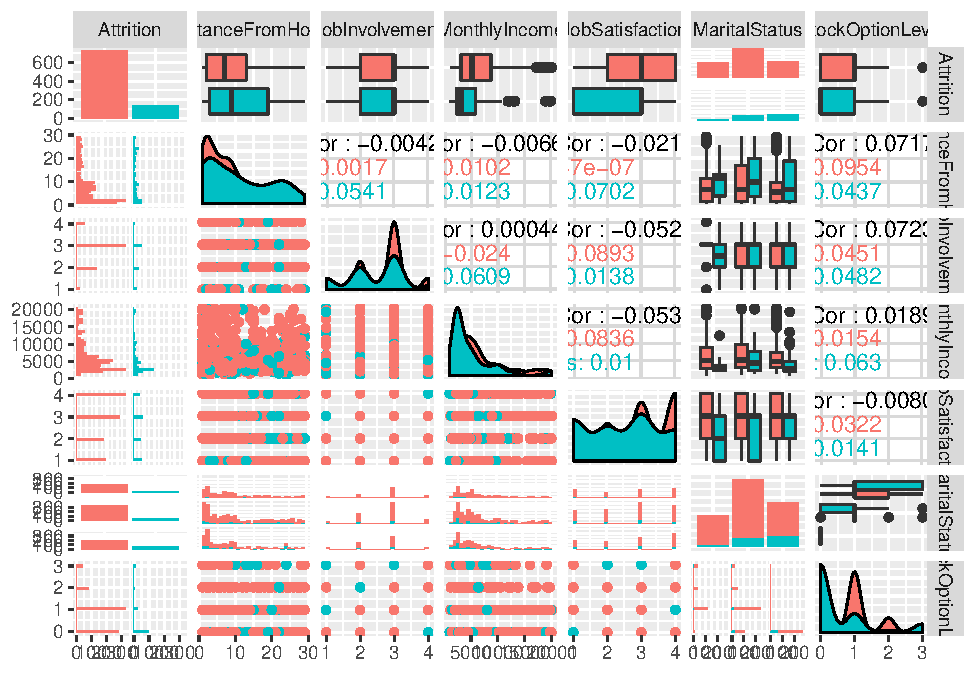
\includegraphics{PresentationPDF_files/figure-latex/unnamed-chunk-5-1.pdf}

\hypertarget{k-nn-classifications-for-attrition}{%
\subsection{k-NN Classifications for
``Attrition''}\label{k-nn-classifications-for-attrition}}

\begin{verbatim}
## Confusion Matrix and Statistics
## 
##      classifications
##        No Yes
##   No  182   2
##   Yes  31   3
##                                          
##                Accuracy : 0.8486         
##                  95% CI : (0.794, 0.8935)
##     No Information Rate : 0.9771         
##     P-Value [Acc > NIR] : 1              
##                                          
##                   Kappa : 0.1186         
##                                          
##  Mcnemar's Test P-Value : 1.093e-06      
##                                          
##             Sensitivity : 0.85446        
##             Specificity : 0.60000        
##          Pos Pred Value : 0.98913        
##          Neg Pred Value : 0.08824        
##              Prevalence : 0.97706        
##          Detection Rate : 0.83486        
##    Detection Prevalence : 0.84404        
##       Balanced Accuracy : 0.72723        
##                                          
##        'Positive' Class : No             
## 
\end{verbatim}

\hypertarget{naivebayes-model-for-attrition}{%
\subsection{NaiveBayes Model for
``Attrition''}\label{naivebayes-model-for-attrition}}

\begin{verbatim}
## Confusion Matrix and Statistics
## 
##      
##        No Yes
##   No  218   2
##   Yes  41   0
##                                           
##                Accuracy : 0.8352          
##                  95% CI : (0.7846, 0.8781)
##     No Information Rate : 0.9923          
##     P-Value [Acc > NIR] : 1               
##                                           
##                   Kappa : -0.0148         
##                                           
##  Mcnemar's Test P-Value : 6.834e-09       
##                                           
##             Sensitivity : 0.8417          
##             Specificity : 0.0000          
##          Pos Pred Value : 0.9909          
##          Neg Pred Value : 0.0000          
##              Prevalence : 0.9923          
##          Detection Rate : 0.8352          
##    Detection Prevalence : 0.8429          
##       Balanced Accuracy : 0.4208          
##                                           
##        'Positive' Class : No              
## 
\end{verbatim}

\hypertarget{predicting-montlyincome-with-linear-regression}{%
\subsection{Predicting ``MontlyIncome'' with Linear
Regression}\label{predicting-montlyincome-with-linear-regression}}

\begin{verbatim}
## 
## Call:
## lm(formula = MonthlyIncome ~ DistanceFromHome + StockOptionLevel + 
##     Attrition + JobLevel, data = flfinal2)
## 
## Residuals:
##     Min      1Q  Median      3Q     Max 
## -5076.5  -913.8    54.7   737.9  3892.4 
## 
## Coefficients:
##                   Estimate Std. Error t value Pr(>|t|)    
## (Intercept)      -1673.829    126.410 -13.241  < 2e-16 ***
## DistanceFromHome   -15.714      5.927  -2.651  0.00816 ** 
## StockOptionLevel    17.438     56.601   0.308  0.75809    
## AttritionYes        30.508    134.023   0.228  0.81999    
## JobLevel          4017.629     44.497  90.289  < 2e-16 ***
## ---
## Signif. codes:  0 '***' 0.001 '**' 0.01 '*' 0.05 '.' 0.1 ' ' 1
## 
## Residual standard error: 1410 on 865 degrees of freedom
## Multiple R-squared:  0.9064, Adjusted R-squared:  0.9059 
## F-statistic:  2094 on 4 and 865 DF,  p-value: < 2.2e-16
\end{verbatim}

\begin{verbatim}
##                        2.5 %     97.5 %
## (Intercept)      -1921.93515 -1425.7221
## DistanceFromHome   -27.34684    -4.0812
## StockOptionLevel   -93.65384   128.5297
## AttritionYes      -232.54079   293.5564
## JobLevel          3930.29357  4104.9641
\end{verbatim}

\hypertarget{conclusion}{%
\subsection{Conclusion}\label{conclusion}}

\begin{itemize}
\tightlist
\item
  Employee Data Analyzed for Predictive Variables
\item
  k-NN computed a better Predictive Model for ``Attrition'' than
  NaiveBayes

  \begin{itemize}
  \tightlist
  \item
    Sensitivity: 85.4\%
  \item
    Specificity: 60\%
  \end{itemize}
\item
  Linear Regression computed an accurate Predictive Model for
  ``MonthlyIncome''

  \begin{itemize}
  \tightlist
  \item
    DistanceFromHome statistically significant (p-value = 0.08)
  \item
    RSME = \$1410
  \item
    Adjusted R-squared: 0.9059
  \end{itemize}
\end{itemize}


\end{document}
